\begin{figure}[H]
	\begin{center}
		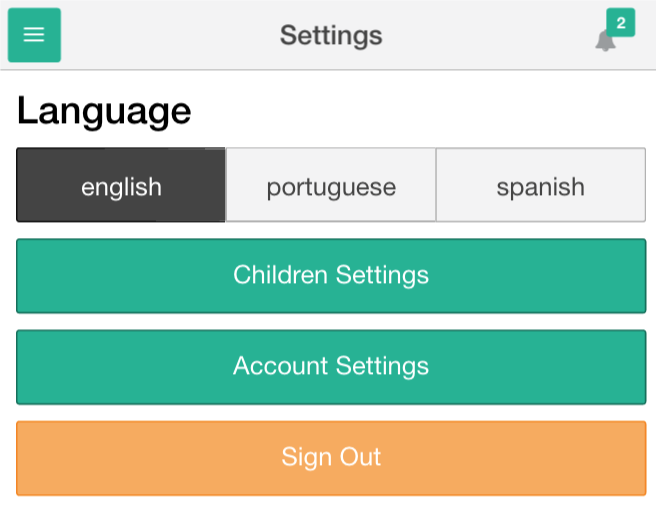
\includegraphics[width=0.5
		\textwidth]{settings/settings_menu.png}
	\end{center}
	\caption{Menu de Configurações}
	\label{fig:9}
\end{figure}

A Figura \ref{fig:9} apresenta as opções de configuração. É possível alterar o idioma, associar filhos à conta do utilizador e alterar informação da conta (ver Figura \ref{fig:9}).

\begin{figure}[H]
	\begin{center}
		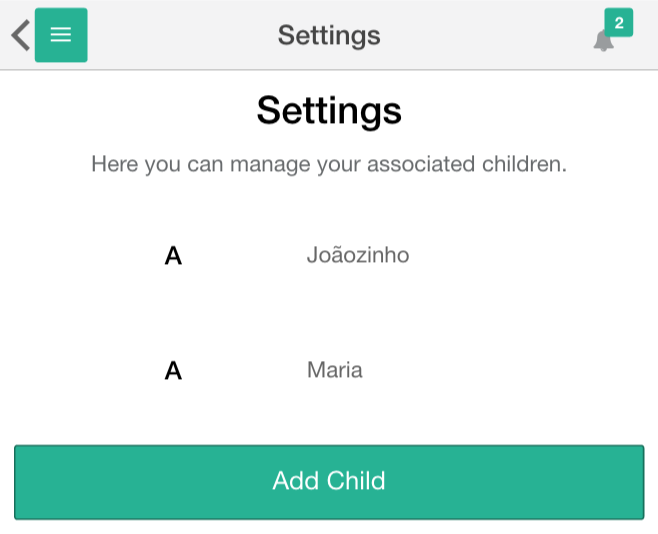
\includegraphics[width=0.5
		\textwidth]{settings/child_settings.png}
	\end{center}
	\caption{Adicionar Filho}
	\label{fig:9_1}
\end{figure}

Para associar um filho é necessário selecionar a opção definição dos filhos, de seguida a opção adicionar filho e por fim inserir o email e password para a conta do filho. Depois o filho pode autenticar-se e utilizar a aplicação.

\begin{figure}[H]
	\begin{center}
		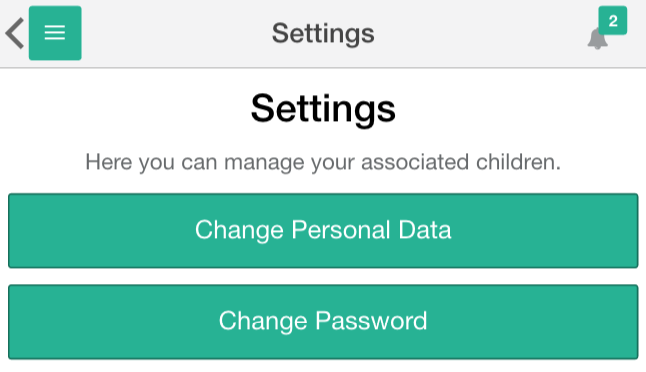
\includegraphics[width=0.5
		\textwidth]{settings/account_settings.png}
	\end{center}
	\caption{Configurar Conta}
	\label{fig:9_2}
\end{figure}

A Figura \ref{fig:9_2} apresenta as opções de alteração da informação da conta: alteração da informação e da \textit{password}. 

\begin{figure}[H]
	\begin{center}
		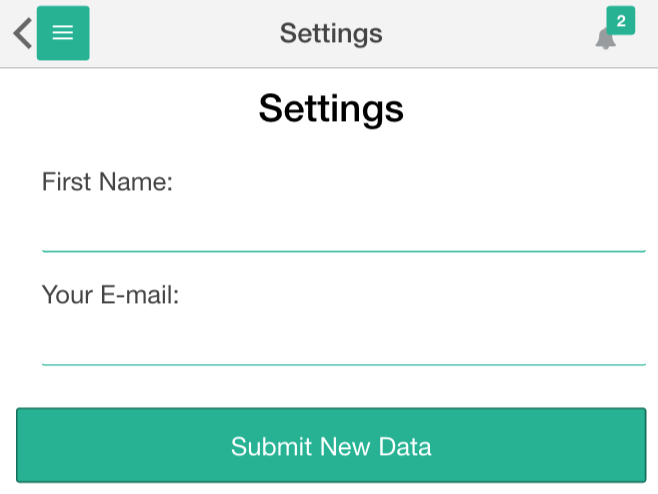
\includegraphics[width=0.5
		\textwidth]{settings/change_account.png}
	\end{center}
	\caption{Alterar Informação da Conta}
	\label{fig:9_3}
\end{figure}

\begin{figure}[H]
	\begin{center}
		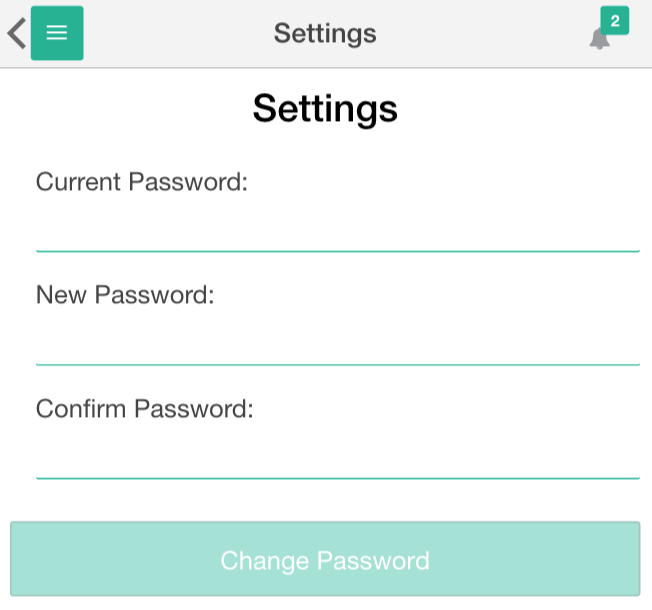
\includegraphics[width=0.5
		\textwidth]{settings/change_password.png}
	\end{center}
	\caption{Alterar \textit{Password}}
	\label{fig:9_4}
\end{figure}

As Figuras \ref{fig:9_3} e \ref{fig:9_4} apresentam, respetivamente, o ecrã de alteração de informação da conta e de alteração da \textit{password}.